\documentclass[pdftex,a4paper]{extarticle}
\usepackage[utf8]{inputenc}

\title{Functional Reactive Programming and its application in Functional Game Programming}
\author{{\large David Kraeutmann, Phillip Kindermann} \\
{\em RWTH Aachen}}

\usepackage{natbib}
\usepackage{graphicx}
\usepackage{url}
\usepackage{amsmath}
\usepackage{amssymb}
\usepackage{amsthm}
\usepackage{enumitem}
\usepackage{minted}
\usepackage{parcolumns}
\usepackage[normalem]{ulem}
\usepackage{multicol}
\usepackage{caption}
\usepackage[a4paper]{geometry}
\usepackage{float}

\usepackage{tikz}
\usetikzlibrary{shapes,snakes}
\usetikzlibrary{scopes,backgrounds}
\usetikzlibrary{fit, positioning}
\usetikzlibrary{calc}

\tikzset{pure function/.style={draw=black, circle, minimum width=3em}}
\tikzset{signal function/.style={draw=black, rectangle, minimum width=3em}}
\tikzset{signal function with state/.style={draw=black, rectangle split, rectangle split parts = 2, rectangle split draw splits = false, minimum width=6em}}

\usepackage{fancyvrb}
\DefineShortVerb{\|}
\VerbatimFootnotes

\begin{document}
\maketitle

\section{Introduction}
Real-time programming is at its core quite imperative --- read input, update state, write output, repeat. 
That requires you to describe \emph{what to do} instead of \emph{what you want}, which leads to a lot of boilerplate when just trying to model a state update.
However, without additional thought even programs written using declarative programming lose their unique benefits due to the imperative style imposed by the update loop, a large amount of state, and discrete-time semantics. 
\begin{listing}[ht]
\inputminted[breaklines=true]{haskell}{Loop.hs}
\captionof{listing}{Update loop of a Haskell program}
\label{lst:imperative}
\end{listing}

To address these issues, Elliott/Hudak formulated \emph{Functional Reactive Programming} (FRP) in \cite{ElliottHudak97:Fran}. FRP evolved in a myriad of different directions and has  applications in robotics, computer vision, animation and games \cite{haskell-wiki-yampa}. 
We'll provide an overview of FRP in Section~\ref{sec:frp}
and focus on Netwire and Elm in particular as implementations in Section~\ref{sec:frameworks}.
A small game written in Elm is presented (Section~\ref{sec:game}) and example implementations of common patterns in game design are discussed.
In (Section~\ref{sec:conclusion}) we provide an overview of benefits and unsolved problems of functional game systems.


\section{Functional reactive programming}
\label{sec:frp}
The core idea of FRP is to provide a set of data types that capture values changing over time. While there are many implementations and approaches to FRP, there are two current approaches: classic and arrows-based functional reactive programming. 

\subsection{Classic FRP}
The initial concept of FRP as used in implementations such as Fran \cite{ElliottHudak97:Fran} or reactive \cite{haskell-wiki-reactive} is based of a few central concepts \cite{conal-what-is-frp,Elliott2009-push-pull-frp}:
\begin{itemize}
\item Time-variant values are first-class, defined similar to \cite{haskell-wiki-frp}
\inputminted{haskell}{Behaviour.hs}
\item Behaviours are created by composing implementation-provided primitives or lifting pure functions into a primitive
\item Discrete phenomena are represented by events
\inputminted{haskell}{Event.hs}
\item For the sake of simplicity and composability, time is assumed to be continuous and discretisation is only introduced when needed.
\end{itemize}

While classical FRP served as an important milestone in the development of reactive programming in a purely functional environment, arrows allowed for a more composable expression of these principles.

\subsection{Arrow-based FRP}
An arrow is a computation that's \emph{like} a function in the sense that it has an input and an output, but is not necessarily a pure function. For example, the usual function type |(->)| is an instance of |Arrow|. You can capture these ideas with a Haskell typeclass taking two type arguments, an input type and an output type, and a set of laws that we'll illustrate using diagrams.
\begin{figure*}[ht]
\centering
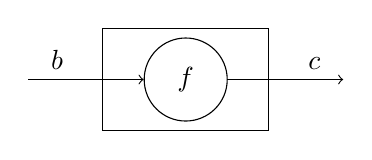
\begin{tikzpicture}[node distance=2cm]
\node[pure function] (pure) {$f$};
\node[signal function, fit=(pure), minimum width=6em] (arrf) {};
\coordinate[left of=arrf] (in);
\coordinate[right of=arrf] (out);
\draw [->, near start] (in) to node[auto] {$b$} (pure);
\draw [->, near end] (pure) to node[auto] {$c$} (out);
\end{tikzpicture}
\caption{arr $f$}
\end{figure*}
\begin{minted}{haskell}
class Arrow a where
    -- Any pure function is a generalised computation
    arr :: (b -> c) -> a b c
\end{minted}

\begin{figure*}[ht]
\centering
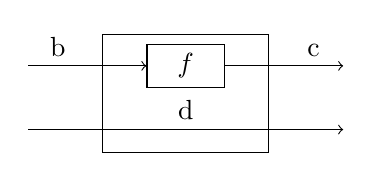
\begin{tikzpicture}[node distance=2cm]
\node[signal function, minimum width=2.8em] (f) {$f$};
\coordinate[below of=f, node distance=2.8em] (lol);
\node[signal function, fit=(f)(lol), minimum width=6em] (arrf) {};
\coordinate[left of=f] (in);
\coordinate[below of=in, node distance=2.3em] (in2);
\coordinate[right of=f] (out);
\coordinate[below of=out, node distance=2.3em] (out2);
\draw [->, near start] (in) to node[auto] {b} (f);
\draw [->, near end] (f) to node[auto] {c} (out);
\draw [->] (in2) to node[auto] {d} (out2);
\end{tikzpicture}
\caption{first $f$}
\end{figure*}
\begin{minted}{haskell}
    -- Apply the computation to part of the input, and ignore the other
    first :: a b c -> a (b,d) (c,d)
\end{minted}

\begin{minted}{haskell}
    -- Computations can be composed similar to (.)
    (>>>) :: a b c -> a c d -> a b d
\end{minted}
\begin{figure*}[ht]
\centering
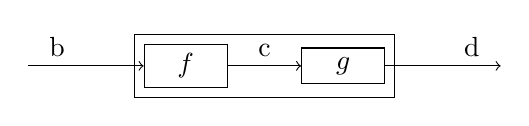
\begin{tikzpicture}[node distance=2cm]
\node[signal function, minimum width=3em] (f) {$f$};
\node[signal function, minimum width=3em, right of=f] (g) {$g$};
\node[signal function, fit=(f) (g), minimum width=6em] (arrf) {};
\coordinate[left of=f] (in);
\coordinate[right of=g] (out);
\draw [->, near start] (in) to node[auto] {b} (f);
\draw [->] (f) to node[auto] {c} (g);
\draw [->, near end] (g) to node[auto] {d} (out);
\end{tikzpicture}
\caption{$f \ggg g$}
\end{figure*}

In our context, this allows us to store opaque (that is, not visible to the user) state along a function in a construct called \emph{signal functions}, which are an instance of |Arrow|.
%Is Netwire a core focus too?
These are used in recent FRP frameworks such as Yampa \cite{hudak2003arrows}, Netwire \cite{haskell-wiki-netwire} and Elm \cite{elm-lang} (albeit in a less rigorous form)  and as such we'll be giving an overview over their usage.

\subsubsection{Signals and signal functions}
\begin{figure}[ht]
\centering
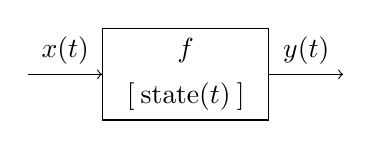
\begin{tikzpicture}[node distance=2cm]
\node[signal function with state, minimum width=6em] (arrf) {$f$ \nodepart{second} $[\: \operatorname{state}(t) \: ]$};
\coordinate[left of=arrf] (in);
\coordinate[right of=arrf] (out);
\draw [->] (in) to node[auto] {$x(t)$} (arrf);
\draw [->] (arrf) to node[auto] {$y(t)$} (out);
\end{tikzpicture}
\captionof{figure}{Signal function}
\label{fig:sigfunc}
\end{figure}

A \emph{signal} is essentially a |Behaviour| from classical FRP --- a value changing over time.
\emph{Signal functions} are, as the name suggests, functions on signals, but also encapsulate state that is only dependent on the input history. State isn't always used; for instance |integral| is a stateful function while |arr| is stateless. That is, the output \(y(t)\) of a stateless function \(f\) is only dependent on the input \(x(t)\), whereas for a stateful function the output depends on a state function \(\operatorname{state}(t)\). This state function summarises the input history \(x(t')\) over the interval \(t' \in [0,t]\). It is also useful that signal functions can inhibit --- that is, produce no value at all --- while still remaining total otherwise (if you were to use |undefined| or a similar bottom type, your program would crash instead).

For the purpose of game programming, we'll present a few combinators that are especially important\footnote{For the sake of simplicity, we'll define |SF a b| as a concrete signal function mapping a to b. Furthermore, we'll use monomorphic types like |Float -> Int| even when the underlying concept is valid for constrained polymorphic types like |Fractional a, Integral b => a -> b|}. It should be noted that this is list is far from exhaustive and is only intended as an overview.

\begin{itemize}
\item In most games, movement input is mapped to change in velocity. In order to convert a velocity signal into a position signal, you need to integrate it: $x(t) = \int_{t_0}^t v(t') dt'$. This is pretty similar to a stateful signal function, and indeed it is. 
\begin{figure}[ht]
\centering
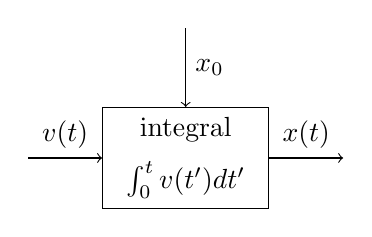
\begin{tikzpicture}[node distance=2cm]
\node[signal function with state, minimum width=6em] (integral) {integral \nodepart{second} $\int_0^t v(t') dt'$};
\coordinate[left of=integral] (in);
\coordinate[right of=integral] (out);
\coordinate[above=1cm of integral] (opt);
\draw [->] (in) to node[auto] {$v(t)$} (integral);
\draw [->] (integral) to node[auto] {$x(t)$} (out);
\draw [->] (opt) to node[auto] {$x_0$} (integral);
\end{tikzpicture}
\end{figure}
For example, you could write \mintinline{haskell}{speed >>> integral 0} to construct a position signal function, and \mintinline[breaklines]{haskell}{gravity >>> integral 0 >>> integral 100} to do the same for a object in free fall from 100m.

\item A set of signal functions operating on intervals\cite{netwire-interval}. For example, \mintinline{haskell}{after :: Time -> SF a b} produces a value after a time period, \mintinline{haskell}{for :: Time -> SF a b} produces a value for a time period, and so on. \mintinline{haskell}{after 60 >>> for 70 >>> gameOver} would give you a 60 second time limit on your game, after which a game over screen displays for 10 seconds (after that the wire inhibits forever).

\item In order to respond to discrete occurences, we use an |Event| type similar to classical FRP. Let's say we want to start moving left when the |A| key is held down. The signal function \mintinline{haskell}{between :: SF (a, (Event b, Event c)) a} inhibits until the left event occurs and then produces until the right event happens. If we define \mintinline{haskell}{keyUp :: SF Key (Event Key)} and an analogous \mintinline{haskell}{keyDown} we can then write something like
\mint{haskell}{moving Left = second (first (keyDown "A") >>> second (keyUp "A")) >>> between}
where \mintinline{haskell}{second} is the same as \mintinline{haskell}{first}, but the other way around.
\begin{figure}[ht]
\centering
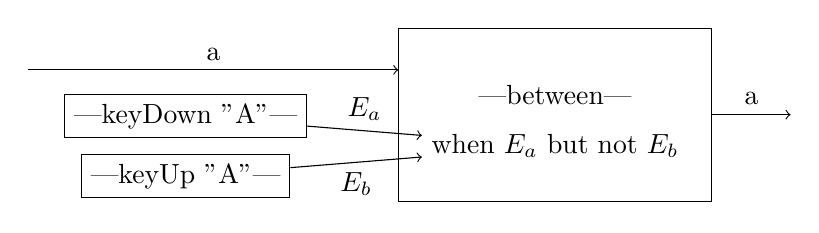
\begin{tikzpicture}[node distance=2cm]
\node[signal function, minimum width=7em] (kd) {|keyDown "A"|};
\node[signal function, minimum width=7em, below=0.2cm of kd] (ku) {|keyUp "A"|};
\coordinate (key) at ($(kd)!0.5!(ku)$);
\coordinate[above=1.25cm of key] (a);
\coordinate[right=3cm of a] (b);
\node[auto, right=3cm of key] (cond) {when $E_a$ but not $E_b$};
\coordinate[below=0.5em of cond] (align);
\coordinate[left=0.5em of cond] (coll);
\coordinate[right=0.5em of cond] (sym);
\node[signal function with state, fit={(b) (cond) (coll) (sym) (align)}] (between) {|between| \nodepart{second}};
\draw[->] (kd) to node[above] {$E_a$} (cond);
\draw[->] (ku) to node[below] {$E_b$} (cond);

\coordinate (reala) at ($(a) + (-2cm,-8pt)$);
\draw [->] (reala) to node[above, midway] {a} (reala-|between.west);

\coordinate[right=1cm of between] (out);
\draw [->] (between) to node[above] {a} (out);
\end{tikzpicture}
\end{figure}
\item All of our previously introduced signal functions can only evolve with time, not be replaced with some other combinator when something happens. For this we use \emph{switching}, with the most important operator being \mintinline{haskell}{(-->) :: SF a b -> SF a b -> SF a b}.
When you have \mintinline{haskell}{f = f1 --> f2}, then \mintinline{haskell}{f = f1} as long as f1 doesn't inhibit. When it inhibits, the signal function permanently switches to \mintinline{haskell}{f = f2}.

As an example let's implement elastic collision with a surface.
\inputminted[breaklines=true]{haskell}{Switch.hs}
The |when| combinator inhibits when the predicate evaluates to |False|, so until we reach the wall's position we move. Once that happens we switch and start moving backwards.

Note that when a switch occurs, local time resets. For example, \mintinline[breaklines]{haskell}{"for 3 seconds" >>> for 3 --> "forever after 6 seconds" >>> at 3} does exactly what the text would lead you to expect.

\item Finally, 
\end{itemize}

\section{FRP frameworks}
\label{sec:frameworks}
\subsection{Netwire}
Not sure if we want to keep this.
\subsection{Elm}
Elm is a basic functional programming language which comes with many features.
One of those features is the Time Traveling Debugger\cite{elm-debugger} which allows the developer of a game to see the change of it over the time and lets him travel forward and backward in his program to seek out bugs.
Another benefit is the feature of hot-swapping\cite{elm-swapping} which allows us to program more interactively as we modify running code.
Those features are combined in the Elm Reactor\cite{elm-reactor} which is a development tool providing us with a strong foundation to maintain our program.
At the core of FRP with Elm is the use of Signals\cite{elm-signal}
\newline
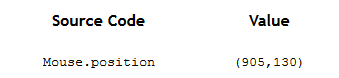
\includegraphics{Signals}
\newline
Basically they are a value that changes over a time but should be rather viewed as a stream of events like our user input or as our state of game.
Elm provides us with a network that processes those signals for us called a signal graph making the use of signals easy.
\cite{elm-examples}

\section{A functional game}
\label{sec:game}

\section{Related works}
\label{sec:related}
Conal Elliott's paper "Push-pull functional reactive programming" \cite{Elliott2009-push-pull-frp} serves an integral role in modern FRP
and serves as the theoretical basis of many FRP libraries. Alexander Berntsen master thesis on programming game systems in Haskell \cite{Berntsen2014-game-systems-haskell} compares imperative and functional game design based on a medium-sized game and provides substantial evidence supporting the usage of strongly static typed purely functional programming for game development. Charles' post about recreating Asteroids in Netwire \cite{asteroids} describes difficulties encountered when implementing a game using Netwire.
\section{Conclusion and Outlook}
\label{sec:conclusion}

\bibliographystyle{plain}
\bibliography{references}
\end{document}